\cotefile{29}
\scanpage{3}
Voorschoten, May 16 1967.\\
Palestrinalaan 11.\\

Dear Grothendieck,\\

I am trying to work out your letter with indications. However I have many difficulties and my progress is very slow. Usually I could find out from your manuscripts for what purpose you developed things in such or such a way, but this time I doubt whether I have grasped the essential points. I can understand your set-up only against the lemma of Abhyankar as background, namely instead of giving directly the covering $\underline{r}(X)$ (in your notation) of $S$, you give the ``behaviour'' of the covering over other coverings, namely the $\underline{s}(M)$, which are of a particular type; apparantly the behaviour over \unsure{a\deleted{l}al|a\deleted{a}ll} these $\underline{s}(M)$ together gives better information then the $\underline{r}(X)$ alone. Is this intuitively a reasonable way of thinking over your new set-up\handwritten{?}

My main difficulty is that I don't see that for a Galois covering the extra structure is uniquely determined. First the concept of Galois covering itself: After the abstract definition and some var\inserted{\handwritten{i}}ations you write: ( I assume that you have a copy) On peut enfin l'expliciter en revenant à la definition de $\mathrm{Rev}^{\underline{R}}(S)$, et en exigeant que les revêtements des $\underline{s}(M)$ correspondants à $X$ soient principaux de groupe $G$. Now in all your examples there is also a group working on the $\underline{s}(M)$, for instance in example 1 a group $\handwritten{\unsure{\mathfrak{g}|g|\mathscr{G}}}$ working on $Z$, and this group acts also on the Galois covering \inserted{\handwritten{corresponding with}} $X$. It seems to me that one must require that the actions of $G$ and $\handwritten{\mathfrak{g}}$ commute; is this correct\handwritten{?} On the same and the next page of your letter you \unsure{explai\deleted{n}m|explai\deleted{m}n} (for example 1) that the functor $\underline{r}$ (geometric realization) is fully faithful (restricted to Galois coverings) under certain conditions; this I don't understand at all ( and \deleted{makes} this makes me feel very uncertain, since I expect that this is an important point \deleted{\unsure{f|i}} if \unsure{\deleted{o}wne|\deleted{w}one} wants to see what is going on\handwritten{!}).

Some other points: in the final formulation of example 3 you introduce a sheme of groups $G(M)$; \deleted{with this formulation} do the objects in example 3a ,with this formulation, consist\deleted{s} out of \uline{couples} $M=(\underline{a},\underline{n})$ and $G(M)=\handwritten{\mu}_{\underline{n}}$ \handwritten{?} Also you write: $\mathrm{Hom}_{\handwritten{\unsure{s|S}'}}(M',M)$ est vide sauf si $\underline{n}'\handwritten{\geq}\underline{n}$, auquel cas....etc....., it seems to me that this sh\handwritten{\tikz[overlay,baseline]{\draw[line width=.4pt] (0,-.02) .. controls (.08,.23) and (.17,.25) .. (.20,.06) .. controls (.22,-.12) and (.36,-.15) .. (.39,-.02);}}uold be ....sauf si $\underline{n}'=\underline{m}.\underline{n}$, auquel cas..... and where $\underline{m}=(m_i)_{i\handwritten{\in}I}$is a a set of positive integers.

\margin{\handwritten{\unsure{,|'}}}
% archive sheet number: 2
\scanpage{4}
\mspage{2.}
I realize that I cause you a lot of trouble and work by asking every time for further explanation and that my assistance in writing the exposé is not very large. Therefore I suggest that you answer this letter only in case it is clear from my questions that I have really a misconception of your new set-up (and it would not surprise me if I have...). Otherwise I shall try to work out your theory as good as I can and make a preliminary manuscript which we can discuss when I am at Bures (I plan to come June 2). In any case, I hope to complete the definit\handwritten{e} version during my stay in Bures.

With kind regards,\\
Sincerely yours,\\
\handwritten{\unsure{J.P. Murre}}\\
% archive sheet number: 3
\scanpage{5}
Voorschoten, March 29 1967\\
Palestrinalaan 11\\

Dear Grothendieck,\\

Enclosed I send you - finally - ,in two different covers, the manuscript on the tame fund. group together with the papers which I borrowed from you.

As to the terminology: I have used scheme in stead of prescheme (without mentioning it because I expect this will be \deleted{\unsure{f}}\inserted{a} general remark in SGA I) but I have not used ``doublet'' because I don't know your final decision on this point.
\margin{\figure{
\begin{tikzpicture}[scale=.8]\node[rotate=35] at (-.65,0) {stroke};\draw (.4,-.25)--(.4,.45);\end{tikzpicture}}}

References: I have made freely references to EGA (also to EGA IV) \uline{but only to SGA 1960/61} (with one notable misleading : a reference to SGA X, Cor 3.3 etc, the purity theorem, is a misleading because the proof is only in SGA 1962). I don't know the `new numbering' of SGA (You mentioned something about it, but I don't remember) so I have used still SGA I, SGA V etc for the 1960/61 séminaire.
\margin{SGA 1}

I must admit that there are still many points which are not satisfactory in the exposition. Below are some comments, motivations and questions:

p.3 Hyp.1\quad Perhaps it would have been nicer to avoid a little longer this assumption. However there is in SGA 1960/61 only a statement about quotients and existence of quotients in case the group is an \uline{ordinary} finite group (it is only in SGA D that the theorems from TDTE III are proved and the proof is long and subtle!) This is the \unsure{reasons|reason} for making the assumption Hyp 1 already here.

p.5. line 6 below:\quad the emphasis on $H$ ordinary group : \unsure{same|some} reason

p.6 (Cor 1.11)\quad \uline{In fact this is a general question} : I have hesitated a little bit with the word ``covering'' for ``revêtement'' (of course: already used in the title!) Originally revêtement was used as translation \deleted{for covering} (in Serre-Lang's paper) for covering (in Lang's paper)! But now there may be confusion with ``covering in some topology'' for instance ``covering in the étale topology'' which is something entirely different. What do you think about this? I don't see what
\margin{\figure{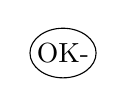
\begin{tikzpicture}[scale=.7]\draw (0,0) ellipse (.6 and .45);\node at (0,0) {\unsure{OK-}};\end{tikzpicture}}}
\margin{OK.}
% archive sheet number: 4
\scanpage{6}
\mspage{2.}
word to use else.

\uline{p.19 etc} : I expected lemma 4.3 to be almost trivial but when I tried to write a proof I did not see an easier one\deleted{\unsure{?}}. Also : the proof of lemma 4.4 is kind of subtle (but this could be expected).
\margin{!}

p.26. line 1:\quad I shall try to find a precise reference.

line 3 :\quad the condition : irreducible in \uline{Zariski topology} is unpleasant but I have not been able to avoid it.

last line in 3) :\quad it seems necessary to mention also the points $s'$.

p.33,34 etc \unsure{..|:}\quad I did not see an easier proof for prop 7.4.

p.43 theor.9.4\quad You have mentioned that the theorem in this form is not satisfactory . for instance the trivial case with constant \unsure{fibres|fibers} and arbitrary crossings escapes. However I don't see how to get a satisfactory statement.

p.45. line 5 etc.\quad Is this indication sufficient?

I have not written an appendix on the Lefschetz theory. If you think this is useful then I can still try.
\margin{\figure{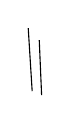
\begin{tikzpicture}\draw (0,0)--(-.05,.8);\draw (.12,-.05)--(.09,.65);\end{tikzpicture}}}

It is not necessary to return the manuscript, I have a carbon copy so you can refer to pages and numbers in your comments. Please give me, if necessary, indications for the way the final manuscript must be typed (is the book a \deleted{foto} photo copy of the manuscript?) Also give me a deadline when you must have the manuscript because I am afraid that I may have already delayed the publication date of your first volume.

With best regards,\\
Sincerely yours,\\
\unsure{J.P. Murre}\\
% archive sheet number: 5
\scanpage{8}
Dear Murre,\\

Thank\unsure{s|x} you very much for your notes ont the tame fundamental group, which I at last finished reading. I see you wrote them with much care, and I am all the more sorry that \unsure{by|hy} my own fault, there is a number of misstatements which, I am affraid, will force you to do a serious recasting of the whole exposition. My notes definitely where too sketchy, and my oral explanations, I am affraid, partly wrong, which induced you into error a few times. Here the most serious drawbacks.

1.16. is false already when $H$ is the unit group and when there is a single $a$, say $a=b^n$, $Y'=Y\ T/(T^n-a)$. Then $Y=S$, and a morphism\deleted{\unsure{s|x}} of $Y$ into $Y'$ compatible with $H=e\quad H'$ is just a section\deleted{\unsure{r|x}} of $Y'$, which exists indeed; however $H\quad H'$ is not surjective. \unsure{\handwritten{3}|3}.6. is equally false, as you see by the previous example, using the given section to define an $H'$-morphism $H'\quad Y'$ which is not an isomorphism\handwritten{!} As a consequence, the proof in your notes of \handwritten{3}.7. breaks down (as it uses 1.16) and so does the proof of \handwritten{3}.8. (I did not try to check \handwritten{3}.8. by some different proof).
% The spaces in Y T, H=e H', H H', and H' Y' are blank in the scan; no bracket or arrow is supplied.

I am affraid \deleted{the proof of} 6.4. is false as stated, and that the statement is correct only if the $D_i$ are regular. Indeed, the end of \unsure{then|the} \deleted{proo\unsure{f}} proof seemed to me very dubious; be careful that the intertia groups are determined only up to interior automorphism ! There is however a \inserted{(tautological)} generalization of the theorem for regular $D_i$, corresponding to the data of a single divisor $D$ with normal crossings, and a variant of the notion of tame ramification for such a divisor, by demanding that the coverings should be tamely ramified locally fot the étale topology for the family of local irreductible components of $D$; it is this notion of tameness which would seem more adapted to the situation of par.9 .
% archive sheet number: 7
\scanpage{9}
\margin{\handwritten{\unsure{11/4/67|17/4/67|11.4.67|17.4.67}}}
The proof of 7.1. is not correct, when you conte\inserted{n}d on line -9: there remains to be proven the following: ... Already when $D=0$, the proof here would have to introduce connected étale coverings which are \uline{not Galois} ! This very strongly suggests that a notion of tame ramification should be introduced also \deleted{in} for non Galois coverings. The same remark applies to the proof of 10.1. Maybe you could get along some way in 7.1. using the normali\deleted{\unsure{x|s}}ty assumptions, but I am convienced that these assumptions are anyhow artificial, as well as the assumption that the $D_i$ should be reduced somewhere. You do not seem to make any use of these facts, really

Also, one feels that 7.\unsure{\deleted{4}5|\deleted{5}4}. should be generalized to the case of a tamely ramified covering, and that it should come out trivially once the generalities have been dealt with properly.

I hope that the theory will come out more clearly and correctly by devoting some care to generalities on ramification data (not necessarily of Kummer type). I will try to write something up within the next days. Please excuse me for the trouble I caused you by not learning my lesson well enough before I put you to work !

It would be very nice indeed to have an appendix on Lefschetz theorem for the tame fundamental group, and it should not be hard to write it. However, if would be safer to wait till the general theory of tame ramification is written up !

Sincerely your's\\
% archive sheet number: 8
\scanpage{10}
\handwritten{24.4\unsure{,|.}67}\\

Dear Murre,\\

I am sending you \unsure{enchosed|enclosed} the sketch which I promised on ramification data, as well as your manuscript together with my annotations. As the paragraphs 1 to 5 will have to be changed entirely, there is maybe not much point for you to look up to carefully my annotations on these. \deleted{As} I would only suggest that you put more \unsure{formmulas|formulas}, arrows etc on \deleted{\unsure{separate}} separate lines, for easier reading; that you normalize the \unsure{stadfard|stanfard|standard} references to SGA, EGA (for instance, no need to indicate SGA when reference is being made to the seminar 1960-61 in which your talk is going to be included itself, reference as (XI 6.1) is then sufficient); that you be cautious when using a locution like ``if primitive $n$.th roots exist over $S$'', which does not mean much by itself, unless you make clear what you really mean. I would propose the following tentative plan for your talk:

\begin{enumerate}[label={}]
\item[1.] Kummer coverings with respect to a given set of sections.
\item[2.] Ramification data.
\item[3.] Properties of the catégory of coverings of type $\underline{R}$. The group ${}_{1}^{\underline{R}}(S,\ )$
% No base glyph is visible before the stacked R and 1; the second argument is blank.
\item[4.] Functorial behaviours.
\item[5.] Galois coverings of type $\underline{R}$.
\item[6.] Abhyankars theorem (for divisors with normal crossings).
\end{enumerate}
etc

The sections 6 to 10 essentially the same as in your notes, just taking into account my observations, and changing inner references according to the changes made in 1. to 5. A paragraph 11 could be an appendix on the tame variant of Lefschetz's theorem. - Par.1 is essentially your previous par.1 ; you should check exactly what is needed in it for \unsure{fhat|what|that}
% archive sheet number: 9
\scanpage{11}
is to follow. Moreover, it would be reasonable to include the fact that when $S$ is normal and the $V(a_i)$ reduced, then the $Z^{\underline{n}}_{\underline{a}}$ are normal (which now is included in your par.5), so that you can refer to this fact when mentionning examples in \deleted{sections}\inserted{par.} 2. to 5. The paragraphs 2 to 5 in this plan correspond approximately to the sections 1. to 4. in my sketchy notes. It will make some work, I am affraid, to put it into shape, but I have the feeling the notions developped with some generality can be useful still in other contexts than just for the kummer type ramification. If you think it would be much simpler to write these sections by restricting throughout to kummer type ramification, please feel free to do so, (and refer to the possible generalization by a suitable remark). I doubt however it will be much simpler, as there are at least two useful variant\unsure{s} of the notion besides the one of your notes (cf ``particular case b '' in my sketch).

Some more specific observations. In theorem 6.4. (which should be formulated, I believe, in terms of tame ramification in the large sense, cf my notes), there is no need to look at the residue characteristics of the non maximal points of the $D_i$. It will turn out a posteriori (and this should be pointed out in a reamrk or corollary) that \deleted{the} if for every maximal point $s$ of every $D_i$, the inertia group at $s$ is prime to the charactéeristic of $k(s)$, then the order of this group must \unsure{by|be} automatically prime to the residue characteristic at any specialization of $s$. (This statement is non empty only when $s$ is of char. zero, of course). In fact, the proof in your notes (after reduction to the strict local case, which is immediate) works out unchanged, provided you observe that if $\unsure{\deleted{\lambda}A|\deleted{A}A|\mathbb{A}|AA}$ is a regular local ring, $(x_i)_{1\ i\ r}$ part of a regular system of parameters, and $(n_i)_{1\ i\ r}$ a system of intergers $\quad1$, not noecessarily
% The spaces in the lower index strings and before 1 have no visible relation signs.
% archive sheet number: 10
\scanpage{12}
prime to the residue characteristic, then the ring $\deleted{B=}$
\[
B=A\ T_1,..,T_r\ /\ (T_1^{n_1}-x_1,\ldots,T_r^{n_r}-x_r)
\]
% No brackets are visible around T_1,..,T_r; the first ellipsis has two dots.
is again regular.

In theorem 7.1. the normality assumptions as well as reducedness assumptions are quite superfluous, only lemme 7.2. is used (which should be stated in paragraph 1, maybe in a single proposition with the analoguous statement concerning normalisty, and properties $(R_k)$ and $(S_k)$ ). On the other hand the proof on page 32 seems to me \deleted{\unsure{uncom|incom}} a little short at one point; I tried to indicate some details in the margin.

As already stated in my notes, the statement of 9.4. is not the most natural one; one should use here the notion of tame ramification in the broad sense (just one divisor $D$ being given, whith normal crossings relatively to $S$). \deleted{This \unsure{w}} The proof would, I guess, require to use the results of sections 7 and 8 in a slightly different form (using the suitable variant of the notion of tame ramification, cf \deleted{\unsure{example|rxample}} particular case b) in my notes). This however does not make any difficulty, in fact the proofs given in 7 and 8 work for any kind of ramification data, provided we assume a statement of the type 7.2. in paragraph 7 .

In 10.2. and 10.3. the significance of the result comes from the fact that the groups considered are just ${}_1(U,\ )$ resp. ${}_1(U,\ )^{(p)}$, and the theorems should be stated accordingly.
% Both group expressions have a blank base before subscript 1 and a blank second argument.

I hope you will be able to get along with these rather sketchy indications. Please \unsure{d\deleted{i}o|d\deleted{o}i} not hesitate to call back on me for whatever does not seem clear to you !

With best wishes,\\
% archive sheet number: 11
\scanpage{79}
Voorschoten, 30-4-69.\\
Palestrinalaan 11.\\

Dear Grothendieck,\\

Last fall I wrote you that I was planning to work out your notes on formal tamely ramified coverings together with a result on ``plumbing''.

In doing so it turned out to be necessary- at least by the method I followed- to write again a lot of preliminaries on tamely ramified coverings, this time for formal schemes. \unsure{l|1|I} am still not ready with the above mentioned ``project''\handwritten{!} Since it took me already much time, I would appreciate it very much to have -before proceeding- your opinion about the \uline{preliminary version} which \unsure{I|1|l} have prepared so far. Of course it is not necessary to read the notes in detail. My question is: what do you think of this set-up and do you think it worthwhile to continue in this way? To me the entire thing seems somewhat indigestible.

I have adjoined some comments on the different chapters. The notes consists of two parts. Part one ( Chap. I-VII) are the preliminaries, part two ( CHap.VIII-X) are your notes and the plumbing. The chapter on the analogue of the theorem of Mumford has still to be written.

I hope you don't mind too much that I bother you again with these tamely ramified coverings\handwritten{!}

With best wishes,\\
Sincerely yours,\\
\handwritten{\unsure{J.P. Murre}}\\
% archive sheet number: 78
\scanpage{80}
\mspage{\handwritten{1.}}

\uline{Comments}.

\uline{Chap.I.} \handwritten{\'}{E}tale morphisms\inserted{of formal schemes} are defined as inductive systems of étale morphisms of usual schemes (1.1.2 and EGA I 10.12.3).

Crucial lemmas: 1.1.6, 1.1.13 and 1.4.9.

As to 1.1.13: étale nbhs for formal schemes are locally completions of étale nbhs of usual schemes. This is used in 7.1.5, itself used in the reduction step 9.3.3.

\uline{Chap.II.} There are Kummer coverings (II-1), generalized Kummer coverings (II-2) and coverings of Kummer type (II-6)\handwritten{!}

No attempt has been made towards completeness; for instance there is no section on the automorphisms of (generalized) kummer coverings.

It would be useful to have a chara\inserted{c}terization of the Algebra of a \uline{generalized} Kummer cov. (cf. with 2.1.8 for Kummer coverings).

\uline{Chap.III.} This is a nuisance\handwritten{!}

I have tried to write only down those things needed for Chap.VIII-X.

It was sufficient to follow the notes which \unsure{\deleted{I}|I} made for usual schemes and therefore I have not followed your new set-up. But one way or the other, one gets the feeling that the notion of tamely ramified covering, although natural, is very unmanageable if one has to use ``the functor'' instead of the geometric realization itself.

Lem\deleted{\unsure{o|c|e}}ma 3.2.11 is a \unsure{techni\deleted{c}val|techni\deleted{v}cal} lemma, used for instance in 3.5.8, 3.6.5 (and \deleted{many} at several places later on).

\uline{Very crucial are} \deleted{are} 3.4.1,3.4.2 ; also the notations introduced there are often used in the sequel.

For 3.5.5 I have given only an indication of the proof; in fact many proofs of III are standard but very unpleasant to spell out in \unsure{a\deleted{l}al|a\deleted{a}ll} details.

Part 3.6 (and especially 3.6.5) are important. Here the geometric realization determines the tamely ramified \unsure{\deleted{v}covering|\deleted{c}vovering}. Usually only normality, instead of regularity, seems to be needed. The difficulty is however that the notion of normality is (perhaps\unsure{)|'} not stable by étale localization (cf.1.7.3 and 1.7.4).

\uline{Chap.VI.} \deleted{\unsure{6|A}} 6.1.3 is used in8.1.9, see\inserted{\handwritten{page}} VIII-8 point c.

6.2.1 and 6.2.2 are technical results, used in the proof that 9.3.5 implies 9.3.2 (see \deleted{\unsure{IX|see}} page IX-17).

% archive sheet number: 79
\scanpage{81}
\mspage{(2).}

\uline{Comments}

\uline{Chap.VII.} This is a technical chapter. The results are delicate , but they are used in an essential way in 9.3 in the reduction step 9.3.3.

As pointed out before: 1.1.13 is used in 7.1.5. In 7.1.5 we have to work with Kummer coverings instead of generalized Kummer coverings; the reason (or at least one of the reasons) is that we don't have an analogous lemma for 2.1.8. As a consequence the assumption $D_i\handwritten{\cap}D_j=\handwritten{\varnothing}$ (see 9.0.1) has to be made.

Also 7.1.6 is a subtle lemma.

\uline{Chap.VIII.} The first page of your notes ``Revêtements formels étales... remark 8.1.6\inserted{i.e. the isomorphism is \uline{canonical}} seems tome to be correct (\handwritten{!}) and essential for 8.1.9.iii.

\uline{Chap.IX.}

\unsure{Th\deleted{i}es|Th\deleted{e}is} is a working-out of yo\unsure{\handwritten{u}r|ur|r} notes.

The assumption $D_{i,\unsure{o|0}}\handwritten{\cap}D_{j,o}=\handwritten{\varnothing}$ is-as p\unsure{\deleted{i}o|\deleted{o}i}inted out above- used in 9.3.3., in order to be able to apply 7.1.6 and 7.1.8 (page IX-13,line 4 top).

\uline{In IX-1} there are several points about which \unsure{I|l|1} am not certain (for instance page IX-4 below). Nevertheless I have used them (\handwritten{!}) because it seems to me that you used them implicitely and without mentioning in your notes and probably these things are more or less standard results in étale cohomology.

\uline{In IX-2} I have not included (yet\unsure{)|'} the proof of the key-theorem 9.2.3.

(this proof is explicit\unsure{\deleted{e}\handwritten{ly}|\handwritten{ly}} given in the letter of Giraud).

\uline{As to IX-3} : the reduction step 9.3.3. seems to me to be very delicate and depends upon the results in chap.VII. (In your notes you give the motivation in the margin \handwritten{!}). It is -in particular- at this point that one has the feeling that the notion of tamely ramified covering is cumbersome.

I hope that part IX-3 is correctly written\inserted{\handwritten{and that I don't have overlooked difficulties}}; I had a lot of trouble with it.

One final remark: I needed here the results on tamely ramified coverings for \uline{usual schemes}; are these included in your planned final version of SGA 1 Exp.XII (see 9.0.4,9.1,4, page IX-6 below)\handwritten{?}

\uline{Chap.X} The plumbing. X-3 is again very cumbersome. It \unsure{\deleted{o}w|\deleted{s}w|\deleted{w}o|\deleted{w}s|w}ould be nicer to work directly with the geometric realization, but there I encountered difficulties, therefore I followed an easy but long way.

% archive sheet number: 80
